\setchapterimage[6cm]{chapter/ship/ship_title_image.jpeg}
\setchapterpreamble[u]{\margintoc}

\setchapterpreamble[u]{\margintoc}
\chapter{Ships and their operators}

\labch{ships}

\section{Abstract}

This chapter focuses on ships in Russia and the world. Ships may have different purposes: military, or civil. Civilian ships are used in a variety of tasks: trucking, fishing, tourism, mineral exploration, rescue work, as well as sports, cultural and other activities. To store a large amount of information about all ships, it is necessary to maintain knowledge bases. One of those knolange bases is Wikidata. This work is aimed at studying the stord in Wikidata objects describing ships and at evaluating the quality and completeness of their properties and descriptions.


\section{Instances of the object "ship"}

\href{https://en.wikipedia.org/wiki/Ship}{A ship} is a large marine vessel.

Object: \href{https://www.wikidata.org/wiki/Q11446}{ship (Q11446)}.
Property: \href{https://www.wikidata.org/wiki/Property:P31}{instance of (P31)}.

Let's build a list of all ships in English with the script in listing \ref{lst:list_of_ship_en}

\begin{lstlisting}[ language=SPARQL, caption={{List of ship in English}\protect\footnotemark}, label=lst:list_of_ship_en, ]
    SELECT ?ship ?shipLabel
    WHERE
    {
      ?ship wdt:P31 wd:Q11446. # instance of ship
      SERVICE wikibase:label { bd:serviceParam wikibase:language "en". }
    }
  \end{lstlisting}
  \footnotetext{\href{https://w.wiki/nDi}{SPARQL-query}, \num{19820} results (2017), \num{50681} results (2020).}

  
\begin{lstlisting}[ language=SPARQL, caption={{List of ship from Russia, Soviet Union and Russian Empire}\protect\footnotemark}, label=lst:list_of_ship_ussr_rf_re_en, ]
    SELECT ?ship ?shipLabel
    WHERE
    {
      ?ship wdt:P31 wd:Q11446. # instance of ship
                                         # ships belongs to:
      { ?ship wdt:P137/wdt:P17 wd:Q34266 } UNION  # Russian Empire
      { ?ship wdt:P137/wdt:P17 wd:Q15180 } UNION  # Soviet Union
      { ?ship wdt:P137/wdt:P17 wd:Q159 }.         # Russia
      SERVICE wikibase:label { bd:serviceParam wikibase:language "en". }
    }
  \end{lstlisting}
  \footnotetext{\href{https://w.wiki/nDk}{SPARQL-query}, \num{107} results (2017), \num{579} results (2020).}

\href{https://www.wikidata.org/wiki/Q281147}{Krasin (1916)} has the biggest quantity of properties according to ProWD report.
  

\section{Bad and good examples}
Good examples of ships on the site of the Wikidata are: \href{https://www.wikidata.org/wiki/Q613128}{SMS Moltke}, \href{https://www.wikidata.org/wiki/Q596282}{HMS Hermes}, \href{https://www.wikidata.org/wiki/Q598079}{HMS Barham}.

Bad examples of ships on the site of the Wikidata were: \href{https://www.wikidata.org/wiki/Q4264229}{Likhoy}, \href{https://www.wikidata.org/wiki/Q18816894}{Nikolay Vilkov}, \href{https://www.wikidata.org/wiki/Q4528362}{SHCH-310}.



\section{Completeness of the Wikidata}
\begin{marginfigure}[0.0cm]
  {
    \setlength{\fboxsep}{0pt}%
    \setlength{\fboxrule}{1pt}%
    \fcolorbox{gray}{gray}{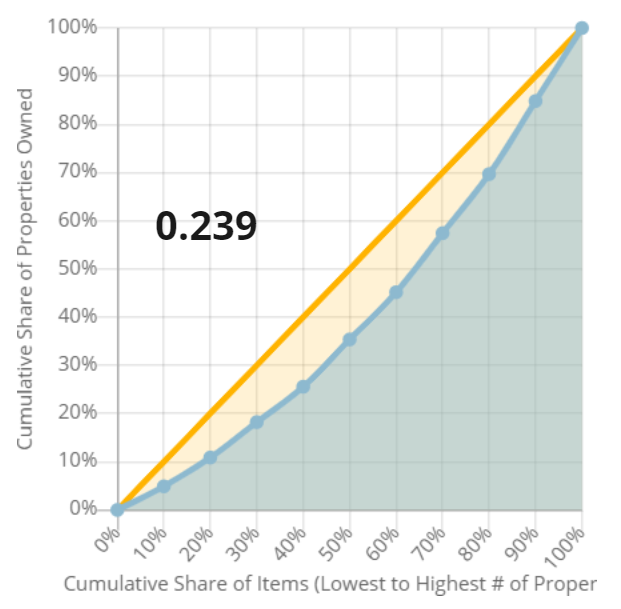
\includegraphics{chapter/ship/Russian_ships_topic_imbalance.png}}
  }
  \caption{
    Wikidata objects' completeness is not uniform:\href{https://www.wikidata.org/wiki/Q11446}{ship (Q11446)}. Data was collected with ProWD.id, 2020. \emph{Gini coefficient is 0.239.}
    }%
    \label{fig:prowd_ships-unbalanced}%
  \end{marginfigure}

Finding the exact number of ships in the world is a difficult task. After all, data about some of them are top secret, some are private vessels and there is no information about them either. Suppose that the total number of ships is 1 210 895, as indicated in the vessel database\footnote{\href{https://en.wikiversity.org/wiki/Research_in_programming_Wikidata/Ships#CITEREFThe_vessel_database2017}{The vessel database 2017}}. \href{https://w.wiki/koU}{SPARQL-query} showed only \num{19886} records, which makes up only 1.6\% of the total number of ships. As for the Russian ships, the actual combat naval personnel of the Russian Navy\footnote{\href{https://en.wikiversity.org/wiki/Research_in_programming_Wikidata/Ships#CITEREFThe_actual_combat_naval_personnel_of_the_Russian_Navy2017}{The actual combat naval personnel of the Russian Navy 2017}} issue 72 submarines, as well as 211 warships and boats. At the time when \href{https://w.wiki/koS}{the query} issued only 25 records. In the first and in the second case, the difference between the actual number of ships and the result of requests is huge, which indicates the incompleteness of the Wikidata. It is also showed by Fig. \ref{fig:prowd_ships-unbalanced}.





\section{Filling the properties of warships}

It is required to find and fill a hundred objects of ships connected with Russia and participating in any military conflicts. Let's do this with the scipt in listing \ref{lst:ships_in_conflict_en}.
\begin{lstlisting}[ language=SPARQL, caption={{List of ships with countries and war conflicts in English}\protect\footnotemark}, label=lst:ships_in_conflict_en, ]
    SELECT ?ship ?shipLabel ?countryLabel ?conflict ?conflictLabel
    WHERE
    {
      ?ship wdt:P31 wd:Q11446;        # instance of ship
            wdt:P137/wdt:P17 ?country;         # belongs to country
            wdt:P607 ?conflict.       # engaged in some conflict
      SERVICE wikibase:label { bd:serviceParam wikibase:language "en". }
    }
\end{lstlisting}
\footnotetext{\href{https://w.wiki/nDo}{SPARQL-query}, \num{1400} results (2017), \num{3586} results (2020).}

When filling the properties of warships, namely the military conflicts in which they participated, the property \href{https://www.wikidata.org/wiki/Property:P607}{conflict (P607)} (war/battle) was indicated. At the same time, military conflicts and military operations, which are part of wars, are different concepts. Filled data on ships can be roughly divided into two types:
\begin{itemize}
  \item \textbf{Objects in which military operations are combined with military conflicts}. For example, in \href{https://www.wikidata.org/wiki/Q4148613}{Soviet destroyer Gremyashchiy} nine wars / battles. Such a large number is due to the fact that the ship took part in many \href{https://en.wikipedia.org/wiki/Arctic_convoys_of_World_War_II}{arctic convoys} which are military operations.
  \item \textbf{Objects in which military operations are separated from military conflicts}. For example, in the British cruiser \href{https://en.wikipedia.org/wiki/HMS_Trinidad_(1940)}{HMS Trinidad} participation in the military campaign and the Arctic convoy are listed as part of World War II with the qualifier \href{https://www.wikidata.org/wiki/Property:P1012}{including (P1012)}. Thus, in the Wikidata, this cruiser has one war/battle.
\end{itemize}

For the first type of filling in the scripts with the search for \href{https://www.wikidata.org/wiki/Property:P607}{conflict (P607)} properties, the ships will display more wars/battles than the second. But in this case, the operation \href{https://en.wikipedia.org/wiki/Siege_of_Odessa_(1941)}{The Odessa Defense} will stand alongside \href{https://en.wikipedia.org/wiki/World_War_II}{World War II}, although it is part of this war. In this situation, the output data will not be accurate.

For the second type of filling, scripts in listing \ref{lst:ships_in_conflict_2_en} will clearly distinguish where the war is, and where the military operation, also the data displayed on the chart will be more accurate.

\begin{lstlisting}[ language=SPARQL, caption={{List of ship with countries and war conflicts in English}\protect\footnotemark}, label=lst:ships_in_conflict_2_en, ]
    SELECT ?ship ?shipLabel ?countryLabel ?conflict ?conflictLabel
    WHERE
    {
      ?ship wdt:P31 wd:Q11446;        # instance of ship
            wdt:P137/wdt:P17 ?country;        # belongs to operator
            wdt:P607 ?conflict.       # engaged in some conflict
      
      { ?country wdt:P17 wd:Q34266 } UNION  # Russian Empire
      { ?country wdt:P17 wd:Q15180 } UNION  # Soviet Union
      { ?country wdt:P17 wd:Q159 }.         # Russia
      
      SERVICE wikibase:label { bd:serviceParam wikibase:language "en". }
    }
\end{lstlisting}
\footnotetext{\href{https://w.wiki/nDn}{SPARQL-query}, \num{105} results (2017), \num{86} results (2020).}


\section{Future work}

\begin{enumerate}
  \item Find the "Guinness ship" (to choose from: the largest, the longest, the most capacious).
  \item Output pictures of those ships, about which the film were shot. If there are no such, then those ships, about which the books were written.
  \item Bring out \href{https://en.wikipedia.org/wiki/List_of_museum_ships}{the museum ships}.
\end{enumerate}


\section{Exercises}

\begin{enumerate}
  \item Based on the graph of the dependence of ships and military operations, which country has the most values of wars associated with ships?
  \begin{itemize}
    \item \href{https://www.wikidata.org/wiki/Q15180}{Soviet Union}
    \item \href{https://www.wikidata.org/wiki/Q159}{Russia}
    \item \href{https://www.wikidata.org/wiki/Q34266}{Russian Empire}
  \end{itemize}
  
  \item Based on the graph of the dependence of ships and military operations, which war accounts for most of the values of ships?
  \begin{itemize}
    \item \href{https://www.wikidata.org/wiki/Q159950}{Russo-Japanese War}
    \item \href{https://www.wikidata.org/wiki/Q362}{World War II}
    \item \href{https://www.wikidata.org/wiki/Q254106}{Crimean War}
  \end{itemize}

  \item The figure \ref{fig:quiz_question_ship} shows the most famous Soviet \href{https://en.wikipedia.org/wiki/Destroyer}{destroyer} \href{https://en.wikipedia.org/wiki/Gnevny-class_destroyer}{project 7}, awarded the title of "Guards", name it.
  \begin{marginfigure}[0.0cm]
    {
      \setlength{\fboxsep}{0pt}%
      \setlength{\fboxrule}{1pt}%
      \fcolorbox{gray}{gray}{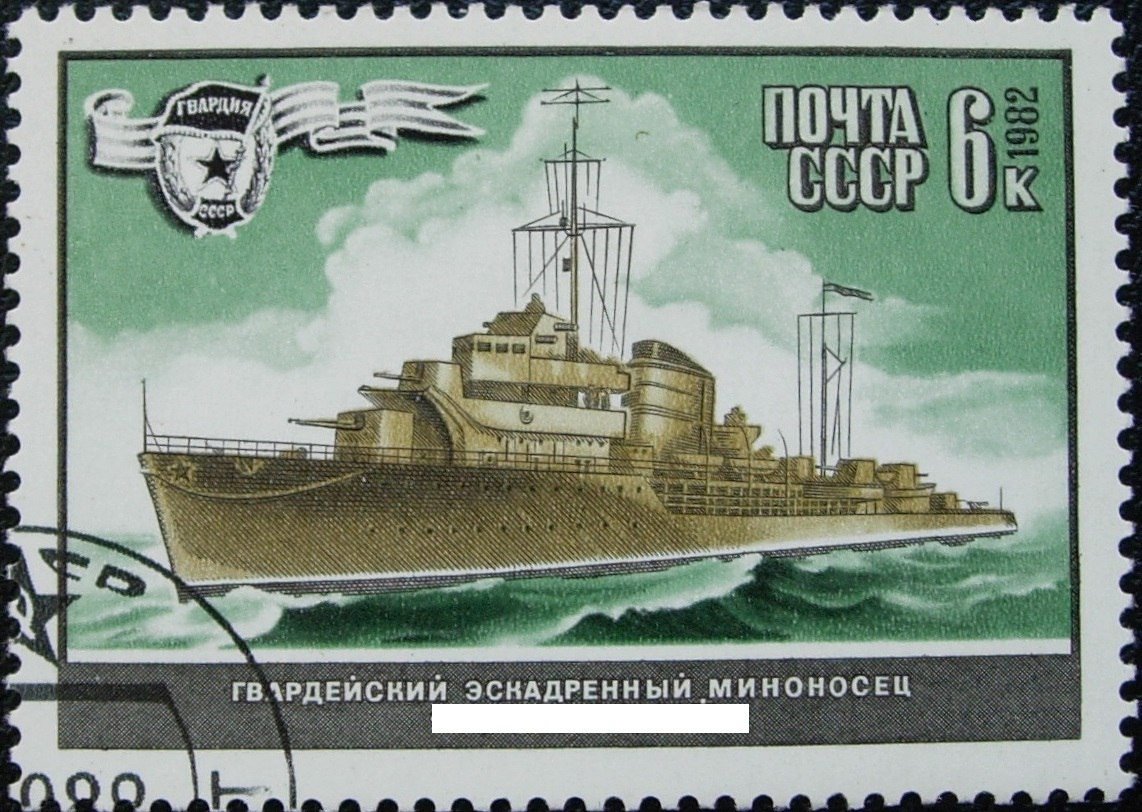
\includegraphics{chapter/ship/Secret_Grem_ship.jpg}}
    }
    \caption{Famous Soviet destroyer project 7.}%
    \label{fig:quiz_question_ship}%
  \end{marginfigure}
\end{enumerate}